\documentclass[aspectratio=169]{beamer}
\usetheme{Madrid}
\usecolortheme{beaver}
\usepackage{fontspec}
\usepackage{listings}
\usepackage{xcolor}
\usepackage{tikz}
\usepackage{fontawesome5}

% Custom colors
\definecolor{agrblue}{RGB}{52, 152, 219}
\definecolor{agrgreen}{RGB}{46, 204, 113}
\definecolor{agrgray}{RGB}{52, 73, 94}
\definecolor{codebackground}{RGB}{248, 249, 250}

% Code style
\lstset{
    backgroundcolor=\color{codebackground},
    basicstyle=\ttfamily\footnotesize,
    keywordstyle=\color{agrblue}\bfseries,
    stringstyle=\color{agrgreen},
    commentstyle=\color{agrgray}\itshape,
    frame=single,
    breaklines=true,
    showstringspaces=false,
    tabsize=2
}

% Title page info
\title{AGR MCP Server}
\subtitle{JavaScript Implementation for Genomics Research}
\author{Development Team}
\institute{Alliance of Genome Resources}
\date{\today}

% Custom title page
\setbeamertemplate{title page}{
    \vbox{}
    \vfill
    \begingroup
        \centering
        \begin{beamercolorbox}[sep=8pt,center,colsep=-4bp,rounded=true,shadow=true]{title}
            \usebeamerfont{title}\inserttitle\par%
            \ifx\insertsubtitle\@empty%
            \else%
                \vskip0.25em%
                {\usebeamerfont{subtitle}\usebeamercolor[fg]{subtitle}\insertsubtitle\par}%
            \fi%
        \end{beamercolorbox}%

        \vskip1em\par
        {\Large \faIcon{dna} \textcolor{agrblue}{JavaScript Implementation} \faIcon{rocket}}

        \vskip1em\par
        \begin{beamercolorbox}[sep=8pt,center,colsep=-4bp,rounded=true]{author}
            \usebeamerfont{author}\insertauthor
        \end{beamercolorbox}
        \begin{beamercolorbox}[sep=8pt,center,colsep=-4bp,rounded=true]{institute}
            \usebeamerfont{institute}\insertinstitute
        \end{beamercolorbox}
        \begin{beamercolorbox}[sep=8pt,center,colsep=-4bp,rounded=true]{date}
            \usebeamerfont{date}\insertdate
        \end{beamercolorbox}\vskip0.5em
    \endgroup
    \vfill
}

\begin{document}

\frame{\titlepage}

% Table of Contents
\begin{frame}{Overview}
    \begin{enumerate}
        \item \textbf{Overview} - AGR MCP Server Features
        \item \textbf{Implementation} - JavaScript Architecture
        \item \textbf{Technical Features} - Key Capabilities
        \item \textbf{Advanced Query Features} - Natural Language Queries
        \item \textbf{Architecture} - High-Performance Design
        \item \textbf{Live Demo} - Installation \& Usage
        \item \textbf{Status \& Future} - Current Status
    \end{enumerate}
\end{frame}

\section{Overview}

\begin{frame}{AGR MCP Server Features}
    \begin{itemize}
        \item \textbf{Enhanced Query Capabilities} \faIcon{search}
            \begin{itemize}
                \item Natural language queries
                \item Boolean logic (AND, OR, NOT)
                \item Species filtering
                \item Cross-entity search
            \end{itemize}
        \item \textbf{Robust Architecture} \faIcon{wrench}
            \begin{itemize}
                \item Node.js implementation
                \item Intelligent caching
                \item Error recovery with backoff
                \item Comprehensive input validation
            \end{itemize}
        \item \textbf{Multiple Interfaces} \faIcon{terminal}
            \begin{itemize}
                \item MCP server for Claude Desktop
                \item CLI tools for command line
                \item Interactive chat interface
            \end{itemize}
    \end{itemize}
\end{frame}

\section{Implementation}

\begin{frame}{JavaScript Implementation}
    \begin{columns}
        \begin{column}{0.5\textwidth}
            \textbf{Core Improvements} \faIcon{star}
            \begin{itemize}
                \item \textcolor{agrblue}{Node.js async I/O}
                \item \textcolor{agrgreen}{Intelligent caching}
                \item \textcolor{orange}{Connection pooling}
                \item \textcolor{purple}{Exponential backoff}
            \end{itemize}
        \end{column}
        \begin{column}{0.5\textwidth}
            \textbf{Advanced Features} \faIcon{magic}
            \begin{itemize}
                \item \textcolor{agrblue}{Natural language queries}
                \item \textcolor{agrgreen}{Boolean operators}
                \item \textcolor{orange}{Multi-entity search}
                \item \textcolor{purple}{Real-time monitoring}
            \end{itemize}
        \end{column}
    \end{columns}

    \vspace{1em}
    \centering
    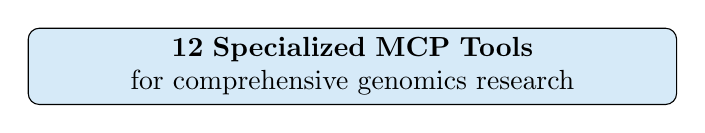
\begin{tikzpicture}
        \node[draw, rounded corners, fill=agrblue!20, text width=8cm, align=center] {
            \textbf{12 Specialized MCP Tools} \\
            for comprehensive genomics research
        };
    \end{tikzpicture}
\end{frame}

\section{Technical Features}

\begin{frame}{Key Capabilities}
    \begin{center}
        \begin{tabular}{|l|l|}
            \hline
            \textbf{Feature} & \textbf{Implementation} \\
            \hline
            Caching & NodeCache with TTL (5-10 minutes) \\
            Rate Limiting & 100 requests/minute per endpoint \\
            Error Handling & Exponential backoff retry \\
            Input Validation & Gene ID and sequence validation \\
            Logging & Structured logging with Pino \\
            Monitoring & Cache hit/miss tracking \\
            \hline
        \end{tabular}
    \end{center}

    \vspace{1em}
    \begin{alertblock}{Architecture Benefits}
        \faIcon{cog} Node.js async I/O with connection pooling for efficient API communication
    \end{alertblock}
\end{frame}

\section{Advanced Query Features}

\begin{frame}[fragile]{Natural Language Queries}
    \textbf{Boolean Logic Support} \faIcon{brain}

    \begin{lstlisting}[language=bash]
# Find DNA repair genes excluding p53 in humans
alliance "breast cancer genes in human AND DNA repair NOT p53"
# Result: 6,021 genes (XRCC3, XRCC1, RAD50, ERCC1, etc.)

# Multiple terms with OR
alliance "insulin OR glucose in mouse"
# Result: 28 genes (Insl5, Igfbp7, Irs3, Ide, etc.)

# Species-specific research
alliance "BRCA1 in human"
# Result: 29 human-specific BRCA1-related genes
    \end{lstlisting}

    \begin{block}{Supported Operators}
        \texttt{AND}, \texttt{OR}, \texttt{NOT} + Species filters (\texttt{in human}, \texttt{in mouse}, etc.)
    \end{block}
\end{frame}

\begin{frame}[fragile]{Cross-Entity Search}
    \textbf{Multi-Dimensional Queries} \faIcon{project-diagram}

    \begin{lstlisting}
// Search genes, diseases, and phenotypes simultaneously
{
  "tool": "complex_search",
  "arguments": {
    "query": "insulin resistance genes and diabetes diseases in human",
    "limit": 10
  }
}

// Advanced faceted search with multiple filters
{
  "tool": "faceted_search",
  "arguments": {
    "genes": ["BRCA1", "BRCA2", "TP53"],
    "diseases": ["breast cancer", "ovarian cancer"],
    "processes": ["DNA repair", "apoptosis"],
    "species": "Homo sapiens"
  }
}
    \end{lstlisting}
\end{frame}

\section{Architecture}

\begin{frame}{High-Performance Architecture}
    \begin{center}
        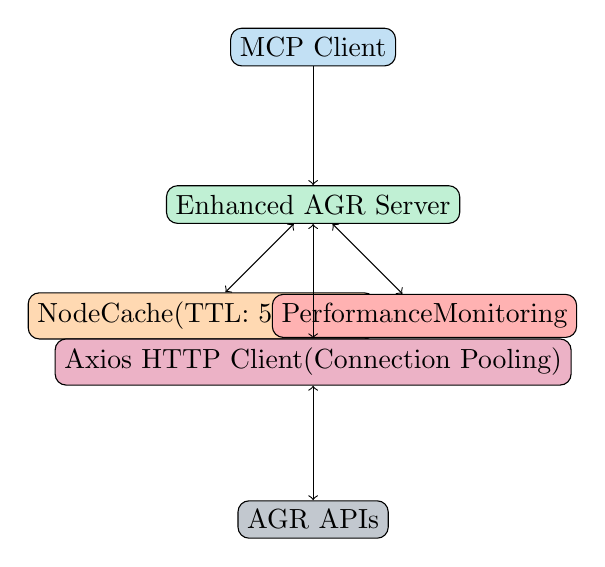
\begin{tikzpicture}[node distance=2cm]
            % Main components
            \node[draw, rounded corners, fill=agrblue!30] (client) {MCP Client};
            \node[draw, rounded corners, fill=agrgreen!30, below of=client] (server) {Enhanced AGR Server};
            \node[draw, rounded corners, fill=orange!30, below left of=server] (cache) {NodeCache\\(TTL: 5-10min)};
            \node[draw, rounded corners, fill=purple!30, below of=server] (http) {Axios HTTP Client\\(Connection Pooling)};
            \node[draw, rounded corners, fill=red!30, below right of=server] (monitor) {Performance\\Monitoring};
            \node[draw, rounded corners, fill=agrgray!30, below of=http] (agr) {AGR APIs};

            % Connections
            \draw[->] (client) -- (server);
            \draw[<->] (server) -- (cache);
            \draw[<->] (server) -- (http);
            \draw[<->] (server) -- (monitor);
            \draw[<->] (http) -- (agr);
        \end{tikzpicture}
    \end{center}

    \begin{columns}
        \begin{column}{0.5\textwidth}
            \textbf{Key Features:}
            \begin{itemize}
                \item Rate limiting (100 req/min)
                \item Automatic retry logic
                \item Input validation
            \end{itemize}
        \end{column}
        \begin{column}{0.5\textwidth}
            \textbf{Monitoring:}
            \begin{itemize}
                \item Cache hit/miss ratios
                \item API response times
                \item Memory usage tracking
            \end{itemize}
        \end{column}
    \end{columns}
\end{frame}

\section{Live Demo}

\begin{frame}{Installation \& Usage}
    \textbf{Quick Setup} \faIcon{rocket}

    \begin{block}{Option 1: npm Package (Recommended)}
        \begin{lstlisting}[language=bash]
# Install globally from npm
npm install -g agr-mcp-server-enhanced

# Available binaries
agr-mcp-server     # Main MCP server
agr-mcp-natural    # Natural language server
alliance           # CLI interface
agr-chat           # Interactive chat
        \end{lstlisting}
    \end{block}

    \begin{block}{Claude Desktop Integration}
        \begin{lstlisting}
{
  "mcpServers": {
    "agr-genomics": {
      "command": "agr-mcp-server",
      "env": { "LOG_LEVEL": "info" }
    }
  }
}
        \end{lstlisting}
    \end{block}
\end{frame}

\begin{frame}[fragile]{Live Examples}
    \textbf{Real Query Results} \faIcon{dna}

    \begin{exampleblock}{PTEN Gene Search}
        \begin{lstlisting}[basicstyle=\tiny\ttfamily]
Query: "find PTEN gene"
Results: 61 genes across species
- PTEN (Homo sapiens) - HGNC:9588
- Pten (Mus musculus) - MGI:109583
- Pten (Drosophila) - FB:FBgn0026379
        \end{lstlisting}
    \end{exampleblock}

    \begin{exampleblock}{Complex Boolean Query}
        \begin{lstlisting}[basicstyle=\tiny\ttfamily]
Query: "breast cancer genes in human AND DNA repair NOT p53"
Results: 6,021 genes (XRCC3, XRCC1, RAD50, ERCC1...)
Performance: <2 seconds response time
        \end{lstlisting}
    \end{exampleblock}
\end{frame}

\section{Status \& Future}

\begin{frame}{Current Status}
    \begin{columns}
        \begin{column}{0.5\textwidth}
            \textbf{Available Features} \faIcon{check-circle}
            \begin{itemize}
                \item \textcolor{agrgreen}{Natural language queries}
                \item \textcolor{agrblue}{Boolean search operators}
                \item \textcolor{orange}{Multi-entity search}
                \item \textcolor{purple}{Comprehensive caching}
            \end{itemize}
        \end{column}
        \begin{column}{0.5\textwidth}
            \textbf{Planned Enhancements} \faIcon{lightbulb}
            \begin{itemize}
                \item JBrowse integration
                \item Batch processing
                \item Additional model organisms
                \item Extended API coverage
            \end{itemize}
        \end{column}
    \end{columns}

    \vspace{1em}
    \begin{alertblock}{Installation}
        \faIcon{download} Available via npm package and Claude Desktop configuration
    \end{alertblock}
</frame>

\begin{frame}{Summary}
    \begin{center}
        {\Huge \faIcon{dna}}

        \vspace{1em}
        {\Large AGR MCP Server - JavaScript Implementation}

        \vspace{2em}
        \begin{columns}
            \begin{column}{0.5\textwidth}
                \textbf{Repository:} \\
                \texttt{agr-mcp-server-js}

                \vspace{1em}
                \textbf{npm Package:} \\
                \texttt{agr-mcp-server-enhanced}
            \end{column}
            \begin{column}{0.5\textwidth}
                \textbf{Architecture:} \\
                Node.js with MCP protocol

                \vspace{1em}
                \textbf{Tools Available:} \\
                12 specialized MCP tools
            \end{column}
        \end{columns}
    \end{center}
\end{frame}

\end{document}